\documentclass[12pt,a4paper,brazil]{abntex2}
\usepackage[utf8]{inputenc}
\usepackage[T1]{fontenc}
\usepackage[brazil]{babel}
\usepackage{graphicx}
\usepackage{lipsum} % Pacote para gerar texto fictício

\titulo{Titulo da Monografia}
\autor{Seu Nome}
\orientador{Nome do Orientador}
\instituicao{%
  Universidade XYZ
  \par
  Faculdade de ABC
  \par
  Curso de XYZ}
\local{Cidade - Estado}
\data{2023}

% Início do documento
\begin{document}

% Capa personalizada
\begin{capa}
    \center
    \ABNTEXchapterfont\Large\textsc{\imprimirinstituicao}

    \vspace*{5cm}

    \ABNTEXchapterfont\bfseries\LARGE\imprimirtitulo

    \vspace*{3cm}

    \Large\imprimirautor

    \vfill

    \large\imprimirlocal

    \large\imprimirdata
\end{capa}

\imprimirfolhaderosto

\sumario % Sumário
\listoffigures   % Lista de Figuras
\listoftables    % Lista de Tabelas

\textual

\chapter{Introdução}
Este é um exemplo de texto com uma nota de rodapé.\footnote{Aqui está o texto da nota de rodapé.} \lipsum[1]

\section{Subtítulo de Nível 1}
Texto com outra nota de rodapé.\footnote{Outro exemplo de nota de rodapé.} \lipsum[2-3]

\subsection{Subtítulo de Nível 2}
\lipsum[4]
\subsubsection{Subtítulo de Nível 3}
\lipsum[5]

\chapter{Revisão da Literatura}
\lipsum[6-7]

\chapter{Metodologia}
\lipsum[8-9]

\chapter{Resultados e Discussão}
\lipsum[10]

\begin{figure}[ht]
\centering
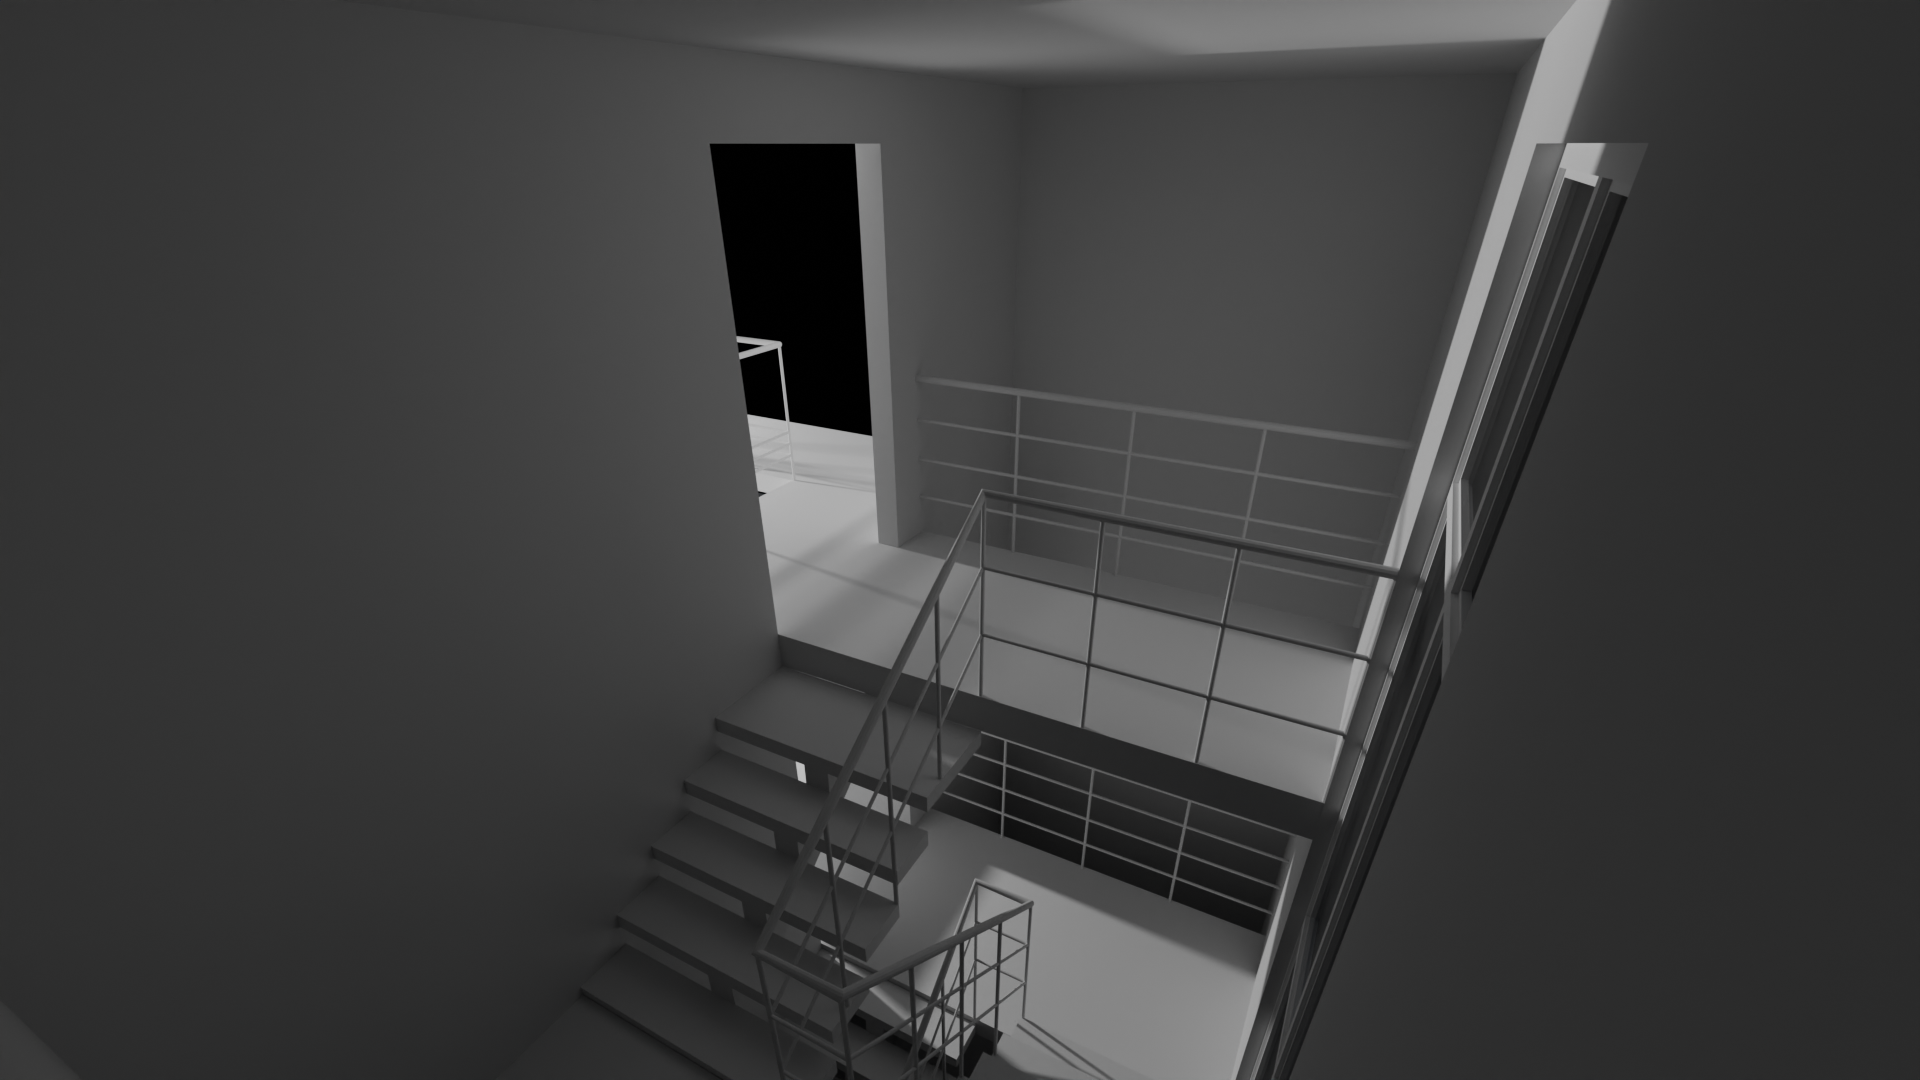
\includegraphics[width=0.5\textwidth]{untitled.png}
\caption{Exemplo de Figura}
\label{fig:exemplo}
\end{figure}

\begin{table}[ht]
\centering
\begin{tabular}{|c|c|c|}
\hline
Coluna 1 & Coluna 2 & Coluna 3 \\ \hline
Item 1   & Item 2   & Item 3   \\ \hline
Item 4   & Item 5   & Item 6   \\ \hline
\end{tabular}
\caption{Exemplo de Tabela}
\label{tab:exemplo}
\end{table}

\chapter{Conclusão}
\lipsum[11-12]

\bibliography{referencias}

\end{document}